\documentclass[12pt, russian, a4paper]{article}

% packages

\usepackage[a4paper, includefoot,
            left=2.5cm, right=1.5cm,
            top=1.5cm, bottom=1.5cm,
            headsep=1cm, footskip=1cm]{geometry}

\usepackage[utf8]{inputenc}
\usepackage[T2A]{fontenc}
\usepackage[english, main=russian]{babel}
\usepackage{graphicx}
\usepackage{amssymb}
\usepackage{amsfonts}
\usepackage{amsmath}
\usepackage{amsthm}
\usepackage{physics}
\usepackage{nicefrac}
\usepackage{cancel}
\usepackage{hyperref}
\usepackage{cmap}
%\usepackage{tempora}
\usepackage{indentfirst}
\usepackage{multirow}

\usepackage{caption}
\usepackage{subcaption}

\usepackage{sectsty}

\sectionfont{\centering\fontsize{12}{12}\selectfont}
\subsectionfont{\centering\fontsize{12}{12}\selectfont}
\subsubsectionfont{\centering\fontsize{12}{12}\selectfont}

\usepackage{setspace}
\onehalfspacing % Полуторный межстрочный интервал
\parindent 1.27cm % Абзацный отступ

\addto{\captionsrussian}{\renewcommand*{\contentsname}{\normalsize\centering СОДЕРЖАНИЕ}}

\addto{\captionsrussian}{\renewcommand*{\refname}{\normalsize\centering СПИСОК ЛИТЕРАТУРЫ}}

\begin{document}
    \begin{titlepage}
	\begin{center}
		{\textbf{\scriptsizeМИНИСТЕРСТВО НАУКИ И ВЫСШЕГО ОБРАЗОВАНИЯ РОССИЙСКОЙ ФЕДЕРАЦИИ}\\
		\textbf{\smallФедеральное государственное автономное образовательное учреждение высшего}\\
		\textbf{образования «Национальный исследовательский Нижегородский}\\
		\textbf{государственный университет им. Н.И. Лобачевского» (ННГУ)}}\\
		\vspace{0.2cm}
		\large{Высшая школа общей и прикладной физики}\\
		\vspace{2cm}
		\Large{\textbf{ГЛОБАЛЬНАЯ АТМОСФЕРНАЯ ЭЛЕКТРИЧЕСКАЯ ЦЕПЬ И КОЛЕБАНИЕ МАДДЕНА--ДЖУЛИАНА}}
	\end{center}
	\vfill
	\begin{singlespacing}
	\begin{tabular}{ll}
		\hspace{8cm} & \begin{tabular}[c]{@{}l@{}} Выпускная квалификационная работа\\ студента 4 курса по направлению\\ подготовки 03.03.02 Физика,\\ профиль – фундаментальная физика,\\ Козлова Александра Владимировича\end{tabular}\\
		& \\
		& \\
		\hspace{8cm} & \begin{tabular}[c]{@{}l@{}}\underline{Научный руководитель}:\\ научный сотрудник ИПФ РАН,\\ кандидат физико-математических наук\\ \\ \underline{\hspace{3.5cm}}Н.Н.~Слюняев\end{tabular}\\
		& \\
		& \\
		\hspace{8cm} & \begin{tabular}[c]{@{}l@{}}\underline{Рецензент}:\\ научный сотрудник ИПФ РАН,\\ доктор физико-математических наук\\ \\ \underline{\hspace{3.5cm}}М.Д.~Токман\end{tabular}\\
		& \\
		& \\
		\hspace{8cm} & \begin{tabular}[c]{@{}l@{}}\underline{Декан~ВШОПФ}:\\ кандидат физико-математических наук\\ \\ \underline{\hspace{3.5cm}}E.Д.~Господчиков\end{tabular}\\
	\end{tabular}
	\end{singlespacing}
	\vfill
	\begin{center}
		Нижний Новгород\\
		2022 г.
	\end{center}
	
\end{titlepage}
    \setcounter{page}{2}

    \tableofcontents
    
    \newpage
    \section*{ВВЕДЕНИЕ}
\addcontentsline{toc}{section}{ВВЕДЕНИЕ}

В земной атмосфере протекают процессы, формирующие климат Земли, что делает изучение атмосферы критически важным для человека. Атмосферное электричество относится к числу наиболее актуальных направлений в науке, изучающей физику атмосферы Земли. Одной из главных задач атмосферного электричества является разработка не противоречащей эксперименту и физически оправданной модели распределения крупномасштабного электрического поля в атмосфере планеты.

Ключевым понятием атмосферного электричества является глобальная электрическая цепь (ГЭЦ) \cite{Williams_Mareev_2014}. ГЭЦ представляет собой распределённый токовый контур, образованный слоем воздуха между землёй и ионосферой. Выделяют два типа ГЭЦ: переменного тока и постоянного. В ГЭЦ первого типа источниками выступают молниевые разряды облако-земля, в ГЭЦ постоянного тока источниками являются токи разделения зарядов в облаках с развитой электрической структурой. Всюду ниже будет рассматриваться ГЭЦ постоянного тока.

Интенсивность ГЭЦ характеризуется ионосферным потенциалом (ИП), который определяется как разность потенциалов между ионосферой и землёй. Замечательной особенностью ИП является то, что он в первом приближении не зависит от географического места измерения. Однако, в последние десятилетия измерений ИП не производится из-за дороговизны таких измерений. Экспериментально измеряется приповерхностный градиент потенциала (ГП) электрического поля Земли, который в дни хорошей погоды пропорционален ИП. ГП в отличие от ИП подвержен множеству локальных эффектов, модулирующих ГП и осложняющих интерпретацию результатов измерений.

ГЭЦ объединяет в себе области плохой погоды, где в среднем электрические токи поднимаются вверх от поверхности земли к ионосфере, и области хорошей погоды, где токи растекаются сверху вниз, поэтому ГЭЦ зависит от климатического состояния Земли. Кроме того, ГЭЦ подвержена влиянию таких факторов космического окружения, как галактические космические лучи и солнечная активность. Так же на ГЭЦ оказывают значительное влияние аэорозоли. Механизмы воздействия данных факторов на ГЭЦ до конца не ясны.%, объяснение механизмов воздействия климатической изменчивости и  на ГЭЦ является актуальной научной задачей.

Аналитическое нахождение распределения крупномасштабных электрических полей в атмосфере в общем случае не возможно, поэтому для исследования ГЭЦ используется численное моделирование. При моделировании ГЭЦ значительные трудности возникают с заданием распределения источников, так как теоретический аппарат, описывающий формирование облака с развитой электрической структурой, не разработан до конца. Модели ГЭЦ разнятся по используемой геометрии, например, некоторые модели рассматривают атмосферу как сферический слой, а в некоторых атмосфера разбивается на невзаимодействующие столбцы воздуха (так называемая столбчатая модель ГЭЦ).

В первой части дипломной работы реализована столбчатая модель ГЭЦ с учётом параметризации проводимости, описанной в \cite{Slyunyaev_et_al_2015}, и параметризации источников, описанной в \cite{Ilin_et_al_2020}. Результаты расчёта ИП, выполненные с помощью данной модели, сравнивались с результатами расчёта ИП по параметризации \cite{Slyunyaev_et_al_2019}. Такое сравнение позволило оценить влияние учёта более точной параметризации проводимости воздуха на моделируемые значения ИП.

%Конвективной деятельностью называют любые проявления конвекции в атмосфере: развитие восходящих и нисходящих токов воздуха, облаков и осадков конвекции, гроз, шквалов, смерчей и тромбов, тайфунов или ураганов и т. д. В метеорологии конвекцию разделяют на мелкую и глубокую [2]. Основное отличие глубокой конвекции от мелкой состоит в том, что она развивается в атмосферном слое большой мощности и важную роль в ее развитии играют процессы, связанные с фазовыми переходами влаги в атмосфере. Другая особенность глубокой конвекции состоит в том, что вследствие больших вертикальных и горизонтальных масштабов существенно возрастает влияние горизонтальной неоднородности метеорологических полей синоптического масштаба, эффекта вращения Земли и неоднородности подстилающей поверхности [8].

Во второй части дипломной работы исследовалась связь колебания Маддена--Джу\-ли\-ана (КМД) с ГЭЦ. КМД является доминирующей компонентой климатической изменчивости в тропиках на временных масштабах в десятки дней. КМД происходит нерегулярно и обычно длится 30--90 дней. Важным аспектом КМД является связанность процессов крупномасштабной атмосферной циркуляции и процессов глубокой конвекции; в течение каждого цикла КМД крупномасштабная связанная структура переносится на восток со скоростью $5\,\textnormal{м с}^{-1}$. Стоит отметить, что к процессам глубокой конвекции относится любая конвективная деятельность, происходящая на достаточно больших вертикальных и горизонтальных масштабах и сопровождающийся процессами, связанными с фазовыми переходами влаги в атмосфере. Эффект переноса конвективной структуры на восток затрагивает все долготы, но наиболее значительное проявление имеет над Восточным полушарием.

За последние 50 лет КМД было широко изучено с климатологической точки зрения \cite{Madden_Julian_1994, Zhang_2005, Zhang_et_al_2020}; было установлено, что КМД воздействует на глобальное распределение дождей, на развитие тропических циклонов и даже на Эль-Ниньо/Южное колебание (ЭНЮК). Однако, лишь несколько исследований было посвящено связям КМД с атмосферным электричеством. В работе \cite{Anyamba_et_al_2000} показано на основе анализа спутниковых данных и измерений резонансов Шумана в Антарктике, что внутри-сезонная вариация глубокой конвекции отражается в вариации интенсивности шумановских резонансов. Резонансы Шумана возбуждаются молниевыми разрядами облако-земля, поэтому не удивительно, что изменение в глубокой конвекции (которая часто связана с молниевой активностью) отражается на их интенсивности. Ещё одно исследование по данной тематике \cite{Beggan_Musur_2019} показывает, что интенсивность и частота резонансов Шумана коррелирует с индексами, описывающими КМД, но только в течение холодной фазы ЭНЮК.

Молниевая активность (а следовательно и шумановские резонансы) связаны с глубокой конвекцией лишь косвенно. Гораздо более естественный подход заключается в рассмотрении ГЭЦ, источниками для которой служат квазистационарные токи разделения зарядов как в грозовых облаках, так и в ESC (electrified shower clouds), в которых нет молний; такие токи непосредственно связаны с глубокой конвекцией.

В недавних работах \cite{Slyunyaev_et_al_2021a,Slyunyaev_et_al_2021b} на основе моделирования ГЭЦ было показано, что изменения в глубокой конвекции в течение ЭНЮК модулирует ИП и его суточную вариацию. Результаты данных исследований нашли подтверждение в экспериментальных измерениях ГП \cite{Harrison_et_al_2011,Slyunyaev_et_al_2021c}. Похожий метод был применён в настоящей работе при исследовании связи ГЭЦ с КМД с использованием как результатов численного моделирования ГЭЦ, так и результатов измерений электрического поля в Антарктиде.
% Что было сделано в этой работе:
% 1) написана столбцовая модель ГЭЦ, обнаружено, что учёт более точной параметризации проводимости никак не сказывается на моделировании ИП по сравнению с моделированием для экспаненциальной проводимости
% 2) КМД и ГЭЦ

    \section{СТОЛБЦОВАЯ МОДЕЛЬ ГЛОБАЛЬНОЙ ЭЛЕКТРИЧЕСКОЙ ЦЕПИ}
    % вывод уравнений на потенциал
    % реализация столбцовой модели ГЭЦ ? (тут про проводимости тинсли)
    % описание модели ГЭЦ с более простой проводимостью ??
    % сравнение двух моделей и оценка нужности учёта более тонкой параметризации проводимости
    \section{ВЛИЯНИЕ КОЛЕБАНИЯ МАДДЕНА--ДЖУЛИАНА НА ГЛОБАЛЬНУЮ ЭЛЕКТРИЧЕСКУЮ ЦЕПЬ}
    \Subsection{ХАРАКТЕРИСТИКА КОЛЕБАНИЯ МАДДЕНА--ДЖУЛИАНА}


    \subsection{МОДЕЛИРОВАНИЕ ГЭЦ С ПРОВОДИМОСТЬЮ, ЗАВИСЯЩЕЙ ТОЛЬКО ОТ ВЫСОТЫ}

В данной части работы использовалась модель ГЭЦ, основанная на параметризации ИП с экспоненциальной проводимостью (см. раздел \ref{sec:exp_sigma}), то есть использовалась формула \eqref{eq:ip}. Для расчета ИП в рамках данной параметризации необходимо задать параметры (высоты изотерм, осадки и CAPE), которые берутся из результатов воспроизведения атмосферной динамики. Для этих целей использовалась модель WRF, позволившая получить требуемые для расчета ИП параметры в виде 24-часового набора данных за каждый третий день с 1 января 1980 года по 29 декабря 2020 года на широтно-долготной сетке 1\textdegree\texttimes1\textdegree. 

%В данной части работы использовалась модель ГЭЦ, основанная на параметризации ИП, предложенной в \cite{Slyunyaev_et_al_2019} на основе идей \cite{Mareev_Volodin_2014}.
%Такая параметризация использует функцию проводимости, которая зависит лишь от высоты $\sigma(z)  = \sigma_0 \exp\qty(z/H)$, и определяет вклады в ИП от каждой ячейки модельной сетки в терминах климатических параметров так, что ИП дается выражением
%\begin{equation}\label{eq:ip}
% 	V = \dfrac{j_0H}{\sigma_0 S_E} \sum\limits_i \qty[\exp\qty(-\dfrac{z^1_i}{H}) - %\exp\qty(-\dfrac{z^2_i}{H})] \times \dfrac{P_i S_i}{W_i} \times \theta(\varepsilon_i - \varepsilon_0),
%\end{equation}
%где $j_0$ --- характерная величина тока разделения зарядов в облаках с развитой электрической структурой, $\sigma_0$ и $H$ приповерхностное значение проводимости воздуха и характерный масштаб увеличения проводимости (в вычислениях полагается $H=6\,\textnormal{км}$), $S_i$ --- площадь, занимаемая $i$-ой ячейкой; $P_i$, $W_i$, $\varepsilon_i$, $z_i^1$ и $z_i^2$ --- общее количество осадков, взятой за симметричный двух часовой интервал, общее количество влаги, максимальное значение convective available potential energy (CAPE) и верхняя и нижняя границы области смешанной фазы в облаке (которые приближались высотами изотерм $0$ \textdegree C и $-38$ \textdegree C) в $i$-ом столбце соответственно, а $\varepsilon_0$ --- граничное значение CAPE, которое полагалось в расчетах $1\, \textnormal{кДж}/\textnormal{кг}$. Сумма (\ref{eq:ip}) берется по по всем столбцам модели. Более глубокий анализ данной формулы производится в \cite{Ilin_et_al_2020}. Важно отметить основные идеи данной параметризации: второй множитель в формуле (\ref{eq:ip}) оценивает площадь, занимаемую облаками в каждой из ячеек модели, а третий множитель позволяет выделить столбцы с развитой конвективной активностью по критерию, основанному на значении CAPE.
%
%Для расчета ИП необходимо задать параметры (высоты изотерм, осадки и CAPE), которые берутся из результатов воспроизведения атмосферной динамики. Для этих целей использовалась Weather Research and Forecasting model (WRF), позволившая получить требуемые для расчета ИП параметры в виде 24-часового набора данных за каждый третий день с 1 января 1980 года по 29 декабря 2020 года на широтно-долготной сетке 1\textdegree\texttimes1\textdegree. 
%
%В итоге были рассчитаны значения ИП за каждый третий день с 1 января 1980 года по 29 декабря 2020 (и вкладов в ИП за тот же период на на широтно-долготной сетке 1\textdegree\texttimes1\textdegree). Значение величины $j_0$ в (\ref{eq:ip}) является параметром модели, оно подбиралось таким образом, чтобы среднее значение моделируемого ИП было равно $240\,\textnormal{кВ}$, что соответствует типичному значению ИП \cite{Markson_2007}.
    \subsection{ИЗМЕРЕНИЯ ЭЛЕКТРИЧЕСКОГО ПОЛЯ НА СТАНЦИИ ВОСТОК}\label{sec:vostok}

За исключением моделирования ГЭЦ с помощью модели WRF в настоящей части работы используются результаты измерений ГП на российской антарктической станции Восток (78.5\textdegree\ ю. ш., 106.9\textdegree\ в. д., $3488\,\textnormal{м}$ над уровнем моря) за период 2006--2020. Такие измерения ГП собираются в удалённом месте и представляют уникальный длинный набор, описывающих ГЭЦ \cite{Burns_et_al_2012,Burns_et_al_2017}.

Электрическое поле измеряется с помощью датчика --- вращающегося диполя, который был установлен на станции Восток в конце 2005 года в рамках российской-австралийского соглашения \cite{Burns_et_al_2017}. Вращающийся диполь установлен на высоте $3\,\textnormal{м}$ на уровнем снежного покрова, возвышаясь над основными строениями станции. Величины ГП собираются в форме усредненных за 10-секундные интервалы значений. По техническим причинам данные имеют большой пропуск во второй половине 2017 года и несколько пропусков поменьше в иное время; кроме того, для некоторых периодов времени доступны только 5-минутные данные.

Чтобы упростить анализ, данные измерений усреднялись по часам UTC, при этом, если доступны как 10-секундные данные, так и 5-минутные данные, брались 10-секундные. При усреднении рассматривались лишь те часы, для которых было записано хотя бы 80\% 10-секундных или 5-минутных значений ГП. Все измеренные значения ГП делились на форм-фактор, равный $3$, для устранения помех, вызванных металлическим стержнем, поддерживающим датчик электрического поля.

Дни хорошей погоды выбирались на основе подхода, примененного в \cite{Slyunyaev_et_al_2021a}. Чтобы выделить дни хорошей погоды, не обязательно использовать метеорологические данные, можно воспользоваться критерием, основанным на значениях ГП, который обычно работает достаточно хорошо \cite{Burns_et_al_2012,Burns_et_al_2017}. Следующая формальная процедура применялась к наборам данных ГП:
\begin{enumerate}
	\item Исключаются дни с неполными или пропущенными часовыми значениями.
	\item Из рассмотрения убираются дни с отрицательными или нулевыми значениями ГП.
	\item Исключаются дни с часовыми значениями ГП, превышающими $300\,\textnormal{В}/\textnormal{м}$.
	\item Среди оставшихся дней удерживаются только те, в которых разница между максимумом суточной вариации и ее минимумом не превышает 150\% от среднесуточного значения.
\end{enumerate}

    \subsection{ЭФФЕКТЫ КМД В МОДЕЛИ ГЭЦ}
\label{sec:eff_mjo_gec}

Чтобы обнаружить паттерны КМД в моделируемой ГЭЦ за период 1980--2020, величины вкладов в ИП усреднялись по дням, отвечающим каждой из восьми фаз КМД. Такие фазы определяются на основе полярного угла на плоскости (RMM1, RMM2) (см. рис. \ref{fig:wh04_fig7}); в среднем в течение цикла КМД точка на данной плоскости движется по окружности вокруг начала координат против часовой стрелки, проходя все фазы. Обычно рассматривают не только фазу, но и амплитуду (расстояние от точки до начала координат), что позволяет разделять КМД на слабое и сильное (см. рис. \ref{fig:wh04_fig7}). В данной работе амплитуда индекса RMM не рассматривалась, так как не было обнаружено какой-либо зависимости в обнаруженных эффектах от нее.

Одной из главных черт КМД является перенос с запада на восток крупномасштабной конвективной структуры в тропиках. Исходя из параметризации ИП (\ref{eq:ip}), вклады в ИП от столбцов модели во многом зависят от CAPE и осадков~---~параметров, связанных с глубокой конвекцией. Поэтому разумно предположить, что паттерны КМД будут заметны во вкладах в ИП.

Так как КМД является нерегулярным процессом, то не следует рассматривать отдельные циклы КМД~---~они могут значительно отличаться друг от друга. Альтернативой такому подходу является переход к некоторому универсальному для КМД временному масштабу~---~масштабу 8 фаз, поэтому среднесуточные значения вкладов в ИП усреднялись по дням, приходящимся на каждую из фаз КМД. Затем вычиталось среднее за длительный период времени значение каждого вклада из усредненных по фазам КМД значений. Таким образом осуществлялся переход к аномалиям вкладов, которые легко интерпретировать: положительная аномалия означает, что данный столбец модели дает вклад в ИП больше, чем обычно, а отрицательная аномалия означает, что вклад данного столбца в ИП ниже обычного значения.

Рис. \ref{fig:map_of_contributions} показывает, как такие аномалии во вкладах меняются с фазой КМД. Видно, что положительная и отрицательная аномалии перемещаются с запада на восток друг за другом с ростом номера фазы КМД. Такой эффект отражает аналогичное перемещение областей усиленной и ослабленной конвективной активности в течение цикла КМД (см. рис. \ref{fig:map_of_olr_anomaly}).

\begin{figure}[tb]
	\centering
	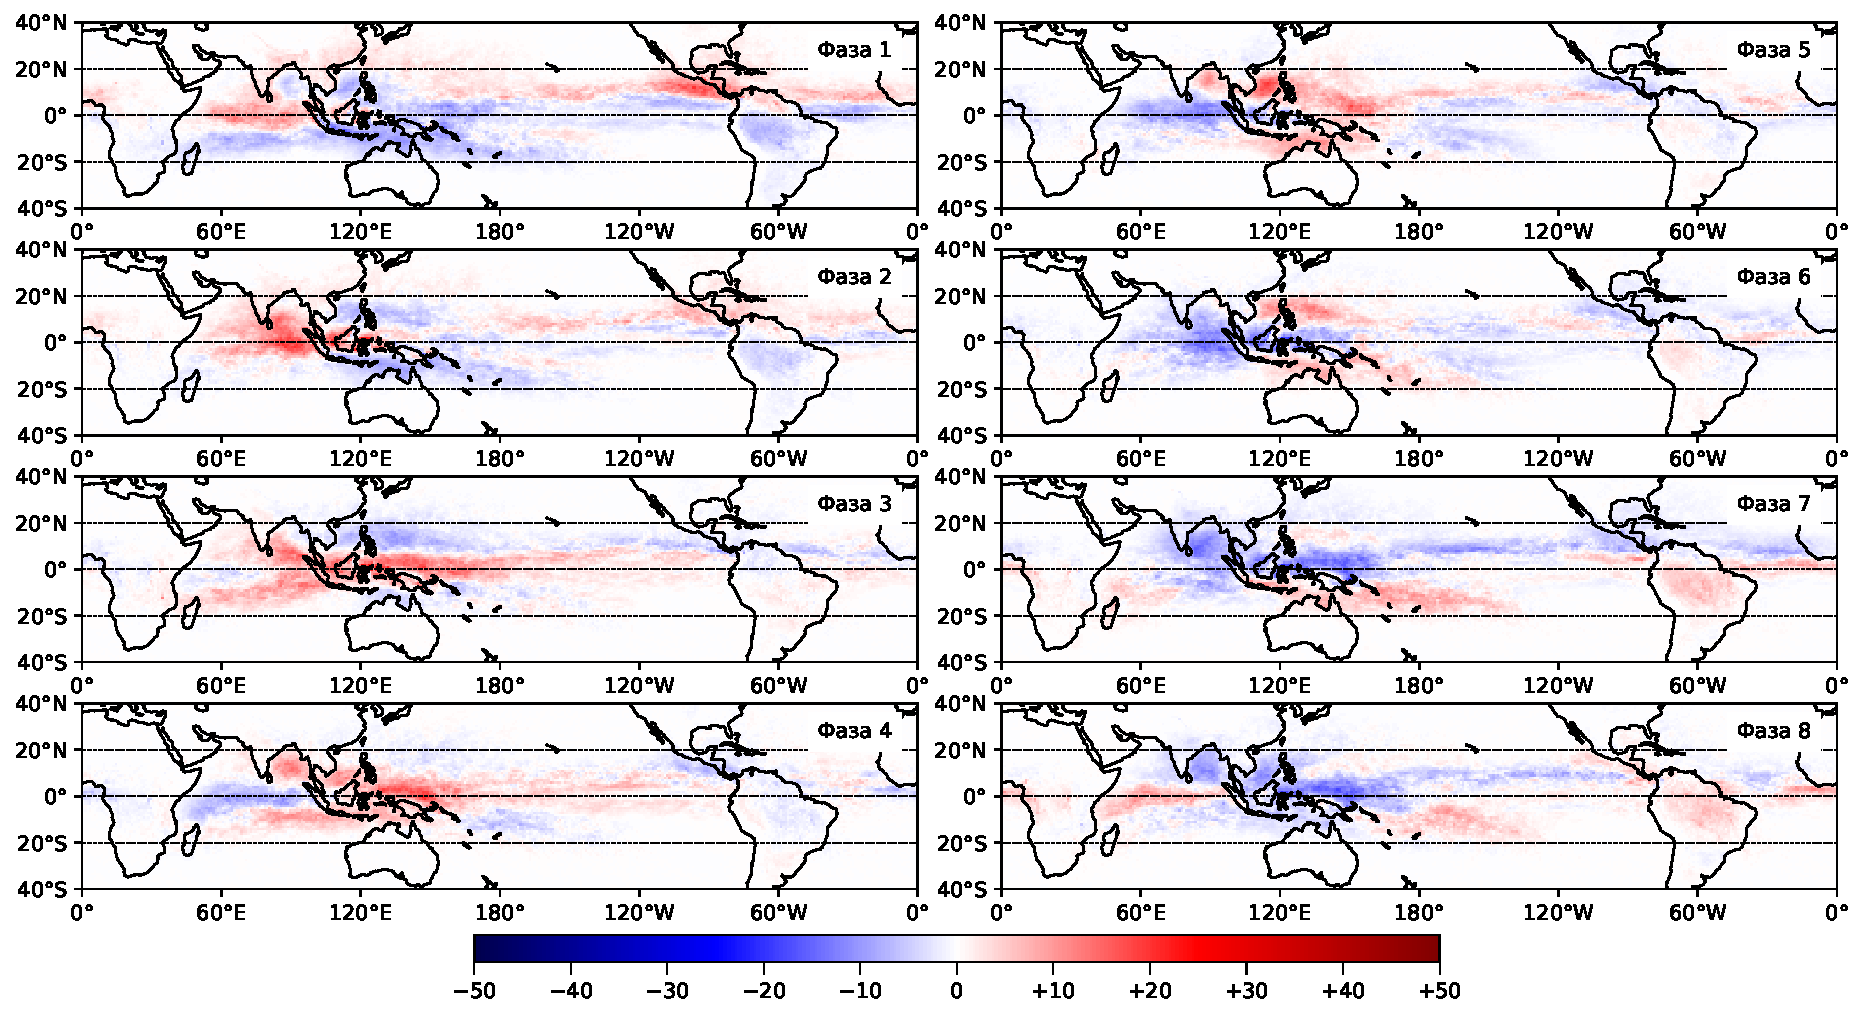
\includegraphics[width=\textwidth]{figures/map_of_contributions.pdf}
	\caption{Аномалии вкладов отдельных модельных столбцов в ИП (в вольтах) в течение каждой из фаз КМД.}
	\label{fig:map_of_contributions}
\end{figure}

Такие образом в среднем моделируемые вклады в ИП изменяются в соответствии с динамикой конвекции на масштабах КМД, что не должно быть удивительным ввиду используемой параметризации (\ref{eq:ip}). Гораздо более интересно было бы посмотреть на такой параметр модели ГЭЦ, как ИП. Рис. \ref{fig:variations}{a} показывает средние значения ИП в различные фазы КМД. Видно, что вариация имеет вид синусоиды с максимумом в фазе 3 и минимумом в фазе 7. Период синусоиды близок к восьми фазам КМД, а амплитуда составляет $12\,\textnormal{кВ}$.

\begin{figure} 
    \centering
    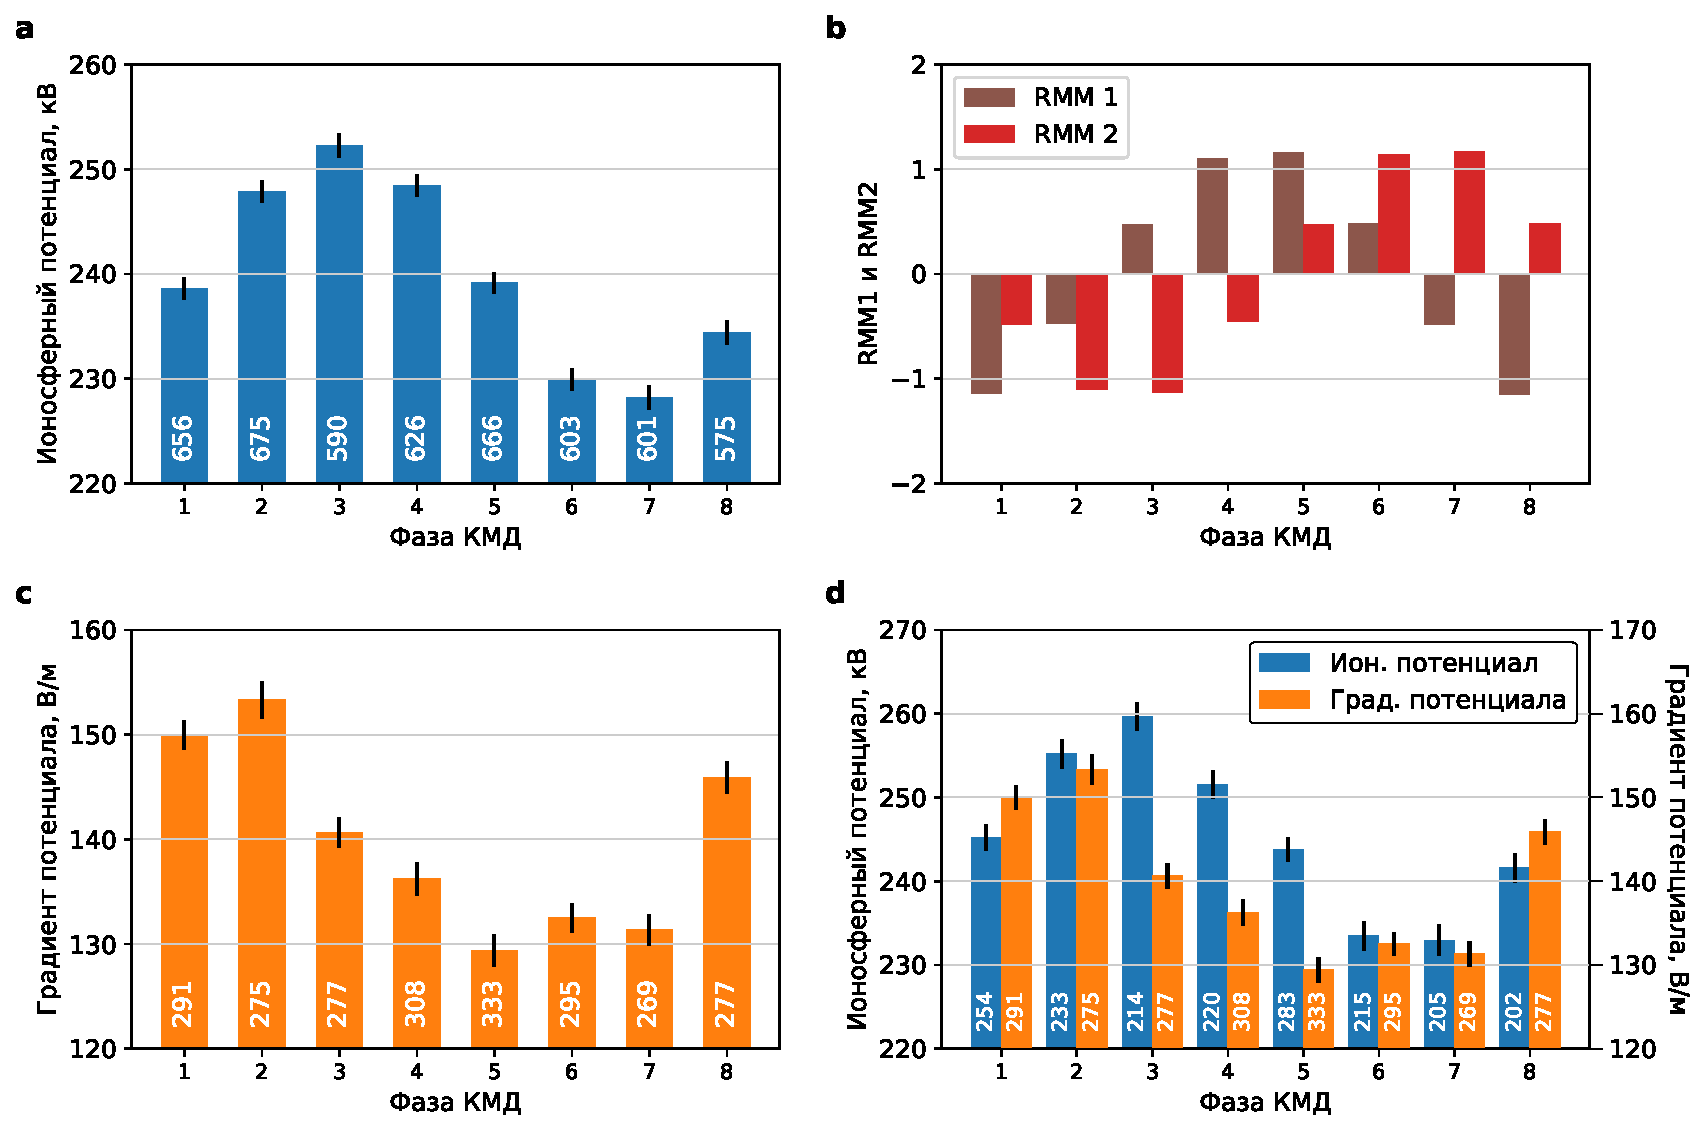
\includegraphics[width=\textwidth]{figures/variations.pdf}
    \caption{(a): Средние значения моделируемого ИП за каждую из фаз КМД (на основе моделирования за 1980--2020). (b): Средние значения компонент индекса RMM за каждую из фаз КМД на основе данных за 1980--2020. (c): Средние значения ГП, измеренного в хорошую погоду на станции Восток, для каждой из фаз КМД (на основе измерений в течение 2006--2020). (d): Сравнение значений ГП, показанных на рисунке (c) со значениями моделируемого ИП за тот же временной интервал (2006--2020). Черные штрихи на столбцах на рисунках (a), (c) и (d) обозначают отклонение в одну стандартную ошибку, а числа в столбцах на тех же рисунках указывают количество дней моделирования или измерений в хорошую погоду, которые пришлись на каждую из фаз КМД.}
    \label{fig:variations}
\end{figure}

Рис. \ref{fig:variations}{b} демонстрирует средние значения RMM1 и RMM2 в различные фазы КМД (на основе данных за 1980--2020). Такие вариации хорошо приближаются синусоидами, ведь фазы КМД возможно определять с помощью полярного угла на плоскости (RMM1, RMM2) (см. рис. \ref{fig:wh04_fig7}), который задается как $\arctg(\mathrm{RMM2}/\mathrm{RMM1})$. Вариации RMM1 и RMM2 имеют схожие амплитуды и сдвинуты друг относительно друга на четверть периода, что отражает тот факт, что усредненная по многим циклам КМД траектория состояния КМД на плоскости (RMM1, RMM2) близка к окружности.

Из сравнения рис. \ref{fig:variations}{b} и \ref{fig:variations}{a} можно заключить, что зависимость ИП от фазы КМД во многом повторяет зависимость величины RMM2, взятой с обратным знаком, от фазы КМД. Точнее, между этими вариациями есть сильная отрицательная корреляция с коэффициентом корреляции $r=-0.93$. В то же время коэффициент корреляции ИП с RMM1 составляет лишь $r=0.33$.

Рассматривается $N = 8$ фаз КМД. Можно оценить значимость наблюдаемой корреляции, используя двухвыборочный t-критерий Стьюдента для независимых выборок с $N - 2 = 6$ степенями свободы. Если даны две независимые выборки размера $N$, а $r$~---~коэффициент корреляции между ними, то величина
\begin{equation}
 	q = \dfrac{r\sqrt{N-2}}{\sqrt{1-r^2}}
\end{equation}
подчиняется распределению Стьюдента. На уровне значимости 1\% гипотеза о том, что две выборки независимы, отвергается, если $q\ge3.71$ или $\abs{r}\ge0.83$. Из данного критерия следует, что отрицательная корреляция между ИП и RMM2 ($r=-0.93$) статистически значима на уровне значимости 1\%, однако связь между ИП и RMM1 ($r=0.33$) не значима.

Если рассматривать данный вопрос более широко, то можно учесть двумерность индекса RMM, что позволяет вместо RMM1 и RMM2 рассматривать проекцию индекса RMM на любое направление в плоскости (RMM1, RMM2), то есть можно оперировать с величиной 
\begin{equation}\label{rmm_direction}
	\mathrm{RMM1}\cdot \cos\phi + \mathrm{RMM2}\cdot \sin\phi,
\end{equation}
где $\phi$~---~полярный угол на плоскости (RMM1, RMM2) (отсчитывается от положительного направления RMM1). Коэффициент корреляции между величиной (\ref{rmm_direction}) и ИП зависит от полярного угла $\phi$ так, как показано на рис. \ref{fig:r} (голубая кривая), и достигает своего максимального значения ($r=0.99$) при $\phi=290^\circ$; на рис. \ref{fig:rmm_diagram} это направление обозначено голубой пунктирной линией. Таким образом, можно утверждать, что значения ИП, будучи усреднены по фазам КМД, крайне хорошо коррелируют с циклом КМД.

\begin{figure}[htbp]
	\centering
	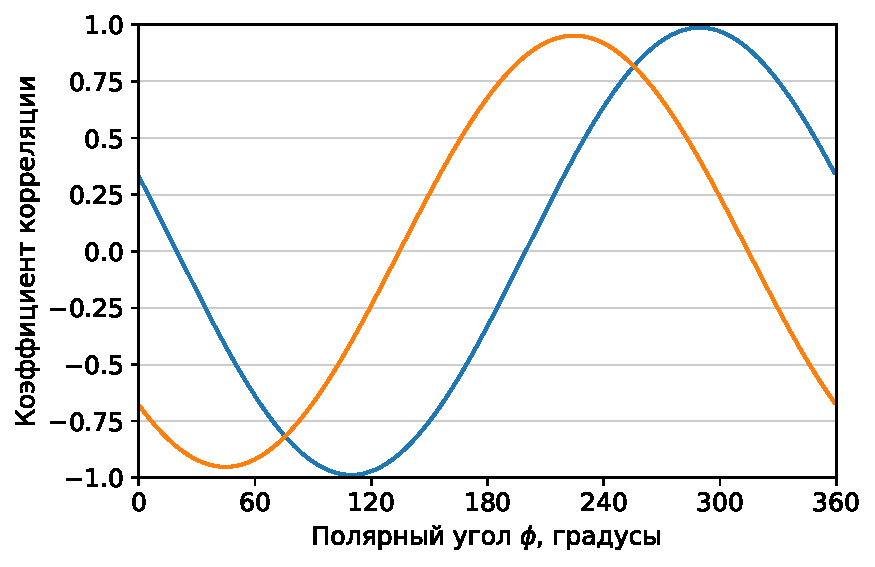
\includegraphics[width=0.6\textwidth]{figures/r.pdf}
	\caption{Коэффициент корреляции между величиной (\ref{rmm_direction}) и ИП (голубая линия), а также между величиной (\ref{rmm_direction}) и ГП (оранжевая линия) в зависимости от полярного угла $\phi$.}
	\label{fig:r}
\end{figure}

Стоит заметить, что направление в сторону отрицательных значений RMM2 соответствует полярному углу $\phi=270^\circ$, что близко к $\phi=290^\circ$, а направление в сторону положительных значений RMM1 соответствует $\phi=0^\circ$, что почти перпендикулярно к направлению $\phi=290^\circ$. Это согласуется с приведенными выше результатами, согласно которым ИП негативно коррелирует с RMM2, но не коррелирует с RMM1.

    \subsection{ЭФФЕКТЫ КМД В РЕЗУЛЬТАТАХ ИЗМЕРЕНИЙ ЭЛЕКТРИЧЕСКОГО ПОЛЯ}

Было показано, что моделируемый ИП имеет синусоидальную вариацию по фазам КМД. Теперь следует исследовать на наличие подобного эффекта результаты измерений ГП на антарктической станции Восток, которые проводились в 2006--2020 (см. раздел \ref{sec:vostok}).

Средние значения ГП, измеренного в хорошую погоду на станции Восток, отвечающие различным фазам КМД продемонстрированы на рис. \ref{fig:variations}{c}. Снова заметна синусоидальная кривая, но менее гладкая, чем та, что получалась для ИП (см. рис. \ref{fig:variations}{a}); вариация ГП имеет максимум в фазе~2 и минимум около фаз 5--7. Точнее, вариация ГП имеет 2 локальных минимума~---~один в фазе~5 и один в фазе~7, которые разделены малым локальным максимумом в фазе~6; однако, так как значения ГП в фазах 5--7 близки, то далее минимумы в фазе~5 и фазе~7 будут пониматься как один минимум.

Если сравнивать динамику моделируемого ИП за 1980--2020 (см. рис. \ref{fig:variations}{a}) и измеренного в хорошую погоду на станции Восток ГП за 2006--2020 (см. рис. \ref{fig:variations}{c}), то можно заметить разницу между двумя такими вариациями. Чтобы сравнение ИП и ГП стало корректным, следует рассматривать значения ГП и значения ИП, усреднённые за одинаковый временной период 2006--2020, что сделано на рис. \ref{fig:variations}{d}. Коэффициент корреляции между двумя вариациями составляет $r=0.50$ (чего не достаточно для статистической значимости на уровне 1\%), но между вариациями присутствует фазовый сдвиг на восьмую часть периода (т.е. на 1 фазу КМД). Если сдвинуть вариацию ГП на 1 фазу вправо, то коэффициент корреляции возрастёт и составит $r=0.90$, чего хватает для статистической значимости на уровне 1\%.

Кроме того, интересно сравнить ГП за дни хорошей погоды с компонентами индекса RMM. Коэффициент корреляции между ГП и RMM1 равен $r=-0.68$, а между ГП и RMM2 коэффициент корреляции составляет $r=-0.67$; ГП одинаковым образом негативно коррелирует с RMM1 и RMM2. Для статистической значимости на уровне 1\% (для чего требуется $\abs{r}\ge0.83$) коэффициенты корреляции слишком малы.

Если рассматривать линейную комбинацию компонент индекса RMM (\ref{rmm_direction}), то коэффициент корреляции между такой линейной комбинацией и ГП, измеренного в дни хорошей погоды, имеет максимальное значение $r=0.95$, что достигается при $\phi=225^\circ$ (см. рис. \ref{fig:r}); такое направление отмечено на рис. \ref{fig:rmm_diagram} оранжевой штрихованной линией. Следует заметить, что такое направление совпадает с биссектрисой третьей четверти фазовой плоскости индекса RMM, что хорошо соотносится с ранними замечаниями о том, что ГП примерно одинаково негативно коррелирует с RMM1 и RMM2. Кроме того, следует отметить, что оптимальное направление для ГП $\phi=225^\circ$ отличается от найденного для моделируемого ИП ($\phi=90^\circ$) на 65\textdegree, что соответствует примерно 1.5 фазам КМД.

Таким образом, было установлено, что как значения ИП, так и значения ГП (усреднённые по фазам КМД) коррелируют с циклом КМД на статистически значимом уровне в 1\%, но их вариации по фазам КМД имеют фазовый сдвиг друг относительно друга. Штрихи на рис. \ref{fig:variations} обозначают плюс и минус одну стандартную ошибку (что равно стандартному отклонению среднего). Из рис. \ref{fig:variations}{d} видно, что несогласие между формами двух вариаций не могут быть объяснены только лишь статистическими ошибками. Другие возможные объяснения различия вариаций заключаются в неточности используемой параметризации ИП, в воздействии локальных эффектов на результаты измерений ГП и в воздействии солнечной активности. Эти вопросы будут обсуждены ниже в разделе ? .
    \Subsection{Детальное обсуждение и объяснение физических механизмов}\label{subsec:2-6}

Так как была обнаружена связь КМД с ИП в том числе и в результатах моделирования ГЭЦ, то возможно проанализировать найденную связь более детально, используя данные вкладов одиночных столбцов модели. В данном подразделе будет предпринята попытка разложить вариацию ИП на простые колебания, чтобы понять физический механизм, лежащий за наблюдаемым эффектом.
    
    % ?? описание используемой модели ГЭЦ %
    % описание измерений ГП на станции Восток %
    % эффекты КМД в ГЭЦ, обнаруженные при моделировании
    % Большой и подробный раздел про объяснение вариации ИП по фазам КМД
    % Эффекты КМД в измерениях ГП
    % обсуждение причин несостыковок

    % ЗАКЛЮЧЕНИЕ

    \newpage
    \addcontentsline{toc}{section}{СПИСОК ЛИТЕРАТУРЫ}
    \bibliographystyle{unsrt}
    \bibliography{inc/references}

\end{document}